
% DARPA CASE

% REPHRASE THIS PARAGRAPH TO AVOID COPYRIGHT CONCERNS
\todo{Rephrase first paragraph - copied from MODELS paper}

In recent years, aerospace stakeholders have realized that avionics systems are subject to possible cyber-attacks just like other cyber-physical systems. Thus, in addition to being fault tolerant, safety-critical avionics systems must also be cyber-resilient. Cyber-resiliency means that the system is tolerant to cyber attacks just as safety-critical systems are tolerant to random faults: they recover and continue to execute their mission function, or safely shut down, as requirements dictate. Unfortunately, systems engineers are currently given few development tools to help answer even basic questions about potential vulnerabilities and mitigations, and instead rely on process-oriented checklists and guidelines. Cyber vulnerabilities are often discovered during penetration testing late in the development process; or worse yet, they may be discovered only after the product has been fielded, necessitating extremely expensive and time-consuming remediation. This is not a sustainable development model. 

The DARPA Cyber Assured Systems Engineering (CASE) program is targeted at developing tools for design, analysis, and verification that enable systems engineers to \textit{design-in} cyber-resiliency for complex cyber-physical systems. 
%
% BRIEFCASE TOOLS AND FEATURES
Our team developed BriefCASE~\cite{case-at-scale}, a tool chain for developing and assuring cyber-resilient embedded systems according to the CASE workflow depicted in Figure~\ref{fig:workflow}. BriefCASE provides a development environment for modeling system architectures in AADL~\cite{feiler-aadl}, analyzing the models for cyber-vulnerabilities, mitigating those vulnerabilities by applying automated model transformations, formally verifying security properties in the model, generating high-assurance component code from model specifications, building the system to a secure kernel target, and finally, generating a system cybersecurity assurance case.  

\begin{figure}[h] 
	\centering 
	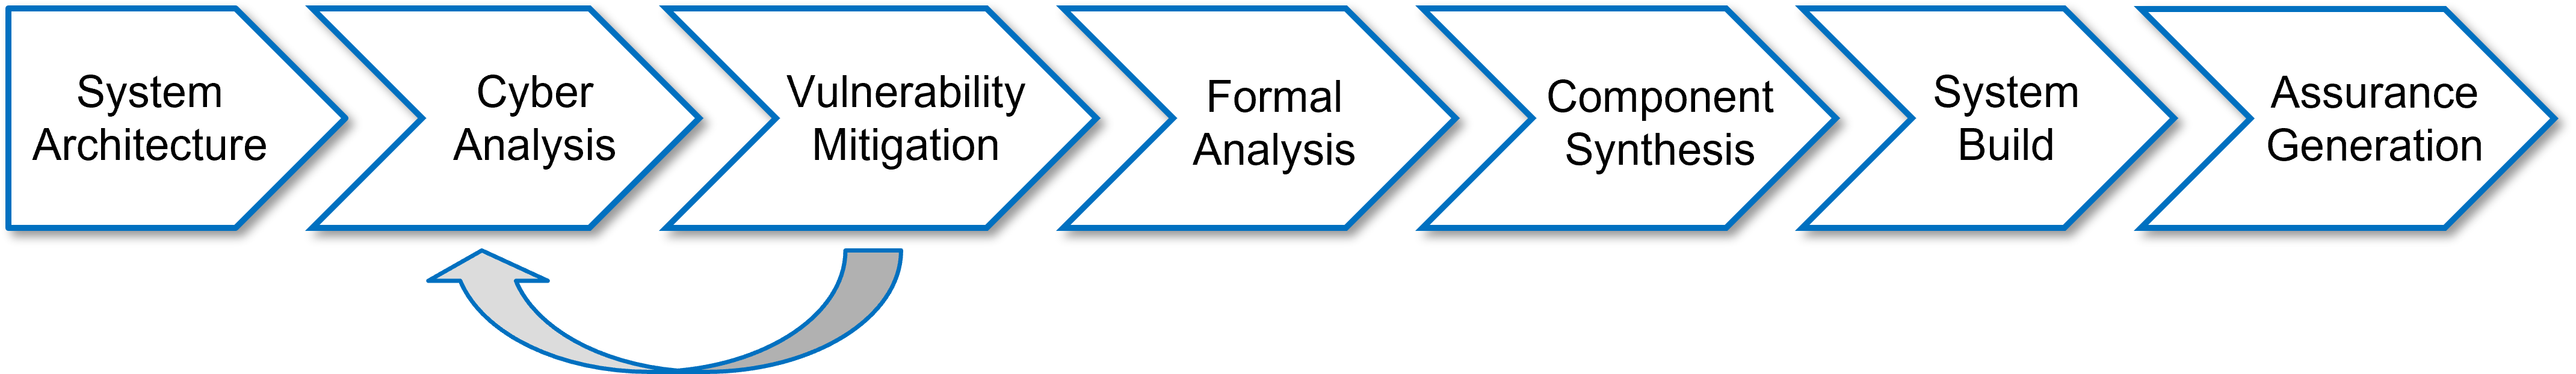
\includegraphics[width=\textwidth]{figs/workflow.png}
	\caption{CASE workflow.}
	\label{fig:workflow} 
\end{figure}

% ASSURANCE
For the development of high-assurance commercial products, there are multiple stakeholders that must be convinced of a product's dependability prior to market-release or deployment.  First and foremost, the developing organization must be confident in the product's correctness.  Next, the certification or accreditation authority must be convinced.  Finally the customer, end user (and often other stakeholders in between) will need to be convinced the product will behave as intended.  Assurance is the process by which an organization compiles a comprehensive argument to demonstrate a product's dependability~\cite{???}.  In order to be effective, the argument must be well-formed, complete, and substantiated with evidence.  Assembling such an argument is not a straight-forward task.  For heavily-regulated environments, it is argued that construction of these arguments should never be left to automation~\cite{???-Holloway}.  In other situations, arguments can be constructed based on assurance templates, or \textit{patterns}, in which generic arguments are defined (ideally arrived at through consensus by a body of experts), then instantiated with a concrete system instance.  This is the approach taken by BriefCASE, which includes a cybersecurity assurance pattern that is instantiated with the system under development, and incorporates evidence produced by artifacts generated by the framework workflow.

% RELATED WORK (Assurance patterns, assurance generation, DMILS, DESTION, what's new here)
\todo{Describe other related work if there's room}

In previous work~\cite{resolute-destion}, we described assurance patterns corresponding to specific BriefCASE mitigations.  However, those patterns primarily focused on assuring aspects of security requirements were satisfied in the model by examining the model structure (for example, demonstrating that an inserted filter component could not be bypassed).  
%
% CONTRIBUTION AND PAPER OUTLINE
In this paper we expand on that work by presenting a comprehensive CASE assurance pattern covering the generation and ingestion of cyber requirements, requirement satisfaction in the model and requirement satisfaction in the realization of the model.  

Section~\ref{sec:assurance-pattern} presents the assurance pattern with respect to the CASE workflow. Specifically, we focus on arguments for security requirement correctness, model correctness, and implementation correctness.  In Section~\ref{sec:evaluation} we describe how the CASE assurance pattern is instantiated and evaluated by the BriefCASE framework.  We provide concluding remarks and discuss future directions in Section~\ref{sec:conclusion}.